\section{Веса IV а}
\subsection{Условие задания}
В графе нет ребер отрицательного веса.

\textbf{Вариант 2:} Определить, есть ли в графе вершина, минимальные стоимости путей от
которой до остальных в сумме не превосходят P.

\subsection{Примеры исходного кода}
Для этой задачи был создан метод \mitext{taskEight()}::
\begin{minted}{typescript}
/**
 * Метод, определяющий, есть ли в графе вершина такая, что сумма
 * длин кратчайших путей от нее до всех остальных вершин
 * не превышает `P`. Построен на основе алгоритма Дейкстры.
 * В графе не может быть отрицательных весов.
 * @param P
 */
taskEight(P: number): boolean {
  /**
   * Вспомогательная функция для определения вершины, до которой
   * путь кратчайший. Возвращает `null`, если пути вообще нет.
   * @param dist расстояния до других вершин
   * @param visited множество посещенных
   */
  const minDistance = (dist: Map<string, number>, visited: Set<string>): string | null => {
    let min = Infinity  // минимальное расстояние
    let minVertex: string | null = null  // метка вершины, до которой расстояние минимальное

    for (const vertex of this.adj.keys()) {
      if (!visited.has(vertex) && dist.get(vertex)! <= min) {
        min = dist.get(vertex)!
        minVertex = vertex
      }
    }

    return minVertex
  }

  /**
   * Алгоритм Дейкстры нахождения кратчайших путей.
   * @param source начальная вершина
   */
  const dijkstra = (source: string): Map<string, number> => {
    const dist: Map<string, number> = new Map()  // расстояния до других вершин
    const visited: Set<string> = new Set()  // для контроля уже посещенных вершин

    // инициализируем расстояния бесконечностью
    for (const vertex of this.adj.keys()) {
      dist.set(vertex, Infinity)
    }

    dist.set(source, 0)  // расстояние до самой себя 0

    for (let i = 0; i < this.adj.size - 1; i++) {
      const u = minDistance(dist, visited)
      if (u === null) {
        break  // если нет путей в непосещенные вершины
      }

      visited.add(u)

      for (const [v, weight] of this.adj.get(u)!.entries()) {
        if (weight < 0) {
          throw new GraphHasNegativeWeights()
        }

        const newDist = dist.get(u)! + weight
        if (newDist < dist.get(v)!) {
          dist.set(v, newDist)
        }
      }
    }

    return dist
  }

  // вычислить сумму длин кратчайших путей для каждой вершины
  for (const vertex of this.adj.keys()) {
    const dist = dijkstra(vertex)
    const sum = Array.from(dist.values())
      .reduce((acc, val) => acc + val, 0)

    if (sum > P) {
      return false
    }
  }

  return true
}
\end{minted}

\subsection{Краткое описание алгоритма}
Алгоритм основан на модификации алгоритма Дейкстры для нахождения кратчайших путей во
взвешенных неориентированных графах.

Вспомогательная функция \mitext{minDistance()}
находит вершину, до которой кратчайшее расстояние и возвращает ее метку.
В случае отсутствия путей в непосещенные вершины возвращает \mitext{null}.

Для каждой вершины графа выполняется алгоритм Дейкстры, который находит кратчайшие
пути от этой вершины до всех остальных. Веса ребер проверяются на отрицательность,
так как алгоритм Дейкстры не будет корректно работать в этом случае.

После нахождения кратчайших путей для каждой вершины вычисляется сумма длин этих
путей. Если сумма превышает заданное значение \mitext{P}, алгоритм возвращает \mitext{false},
иначе \mitext{true}.

\subsection{Примеры входных и выходных данных}
\subsubsection{Входные данные}
\begin{figure}[H]
  \begin{minipage}{0.5\textwidth}
    \centering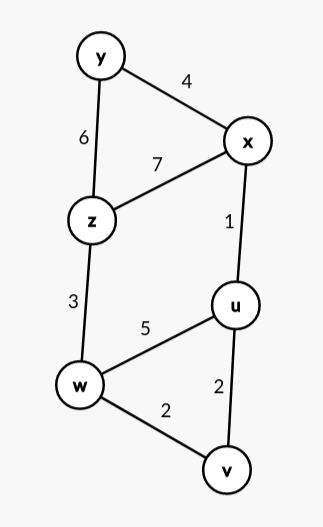
\includegraphics[width=0.6\linewidth]{figs/task-8/graph-8.png}
  \end{minipage}
  \begin{minipage}{0.5\textwidth}
    \centering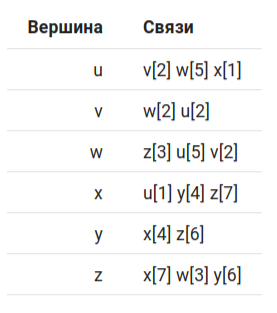
\includegraphics[width=0.6\linewidth]{figs/task-8/adj-8.png}
  \end{minipage}
  \caption{Взвешенный граф}
\end{figure}

\begin{minted}{js}
{
  "weighted": true,
  "oriented": false,
  "adj": {
    "u": {
      "v": 2,
      "w": 5
    },
    "v": {
      "w": 2
    },
    "w": {
      "z": 3
    },
    "x": {
      "u": 1
    },
    "y": {
      "x": 4,
      "z": 6
    },
    "z": {
      "x": 7
    }
  }
}
\end{minted}

\subsubsection{Выходные данные}
\begin{figure}[H]
  \begin{minipage}{0.5\textwidth}
    \centering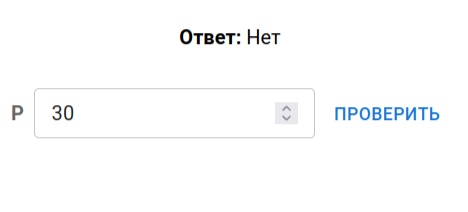
\includegraphics[width=0.8\linewidth]{figs/task-8/res-8-1.png}
  \end{minipage}
  \begin{minipage}{0.5\textwidth}
    \centering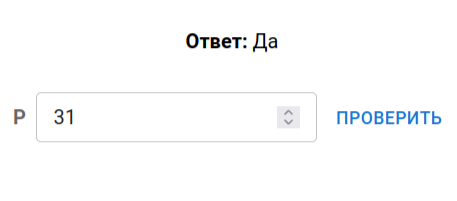
\includegraphics[width=0.8\linewidth]{figs/task-8/res-8-2.png}
  \end{minipage}
  \caption{Результат работы}
\end{figure}